\documentclass{beamer}

% choose theme (warning, to use the UniBern theme you need to copy the files beamerthemeUniBern.sty and ublogo.pdf in the same directory)
\usetheme{UniBern}

% packages

\usepackage{graphicx}
\usepackage{hyperref} % allows clickable urls
\usepackage{tikz}
\usepackage{listings} % show code
\usepackage{dsfont} % show code
\usepackage{fontawesome}
\usepackage{tikz}

% slide numbering
\setbeamertemplate{sidebar right}{}
\setbeamertemplate{footline}{%
	\hfill\usebeamertemplate***{navigation symbols}
	\hspace{1cm}\insertframenumber{}/\inserttotalframenumber}

% define title page
\title{Bayesian workflow for disease transmission modeling in Stan}
\subtitle{{\small Eustat -- XXXIII International Statistical Seminar} }
\author{Julien Riou, MD PhD}
\date{Institute of Social and Preventive Medicine, University of Bern, Switzerland}
\institute{institute}


% begin document
\begin{document}

\frame{\titlepage}

\frame{
	\frametitle{Preface}
	\begin{itemize}
		\item Objective: fit transmission models in Stan 
		\item Based on Grinsztajn et al., 2020 (\underline{\href{https://arxiv.org/abs/2006.02985}{link}})
		\item Prerequisites:
			\begin{itemize}
				\item general understanding of Bayesian inference
				\item basic programming with \texttt{R} and \texttt{Stan 2.21} 
			\end{itemize}
		\item All material is available on \url{https://github.com/jriou/bayesian_workflow}
	\end{itemize}
}

\frame{
	\frametitle{Outline}
	\begin{itemize}
		\item \textbf{Introduction}
		\item (Quick notice: Bayesian inference with Stan)
		\item Fitting a simple SIR
		\item Simulations to understand the model
		\item Scaling up ODE-based models
		\item Extensions 
	\end{itemize}
}

\frame{
	\frametitle{Introduction}
	Models of disease transmission:
	\begin{itemize}
		\item Interpretability: \alert{mechanistic}, phenomenological
		\item Scale: agent-based, \alert{population-based}
		\item Framework: \alert{deterministic}, stochastic
		\item Data-generating mechanisms: incubation, contagion, immunity...
	\end{itemize}
	\pause
	
	\vspace{2em}
	Mechanistic + population-based + deterministic 
	
	\vspace{1em} $\rightarrow$ \alert{ordinary differential equations (ODE)-based compartmental model} 
}

\frame{
	\frametitle{Introduction}
	ODE-based compartmental model:
	\begin{itemize}
		\item Divide the population into homogeneous groups (\alert{compartments})
		\item Define the \alert{flows} between compartments with ODEs
		\item Define initial conditions (at $t_0$)
		\item Solve for the time-dependent volume in each compartment
	\end{itemize}
	\vspace{1em}
	\pause
	
	The \alert{susceptible-infectious-recovered} (SIR) model:
	\begin{figure}
		\centering
		\scalebox{.8}{
		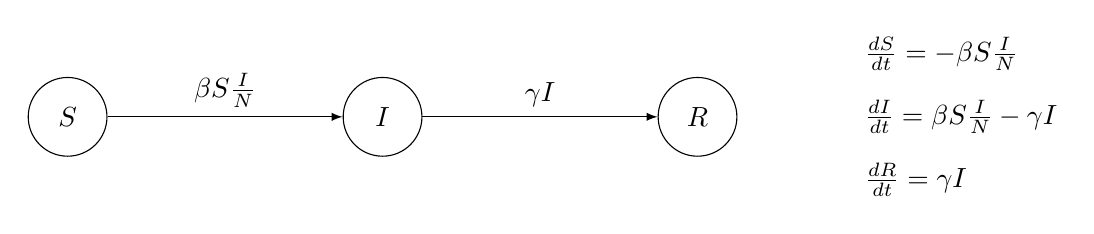
\begin{tikzpicture}
			\node[circle, draw, inner sep=0pt, minimum size=1cm] (S) at (0,0) {$S$};
			\node[circle, draw, inner sep=0pt, minimum size=1cm] (I) at (4,0) {$I$};
			\node[circle, draw, inner sep=0pt, minimum size=1cm] (R) at (8,0) {$R$};
			
			\draw[->,>=latex] (S) edge node[above] { $\beta S \frac{I}{N}$} (I);
			\draw[->,>=latex] (I) edge node[above] { $\gamma I$} (R);
			
			\node[anchor=west] at (10,.8) {$	\frac{dS}{dt} = - \beta S \frac{I}{N}$};
			\node[anchor=west] at (10,0) {$	\frac{dI}{dt} = \beta S \frac{I}{N} - \gamma I $};
			\node[anchor=west] at (10,-.8) {$\frac{dR}{dt} = \gamma I $};
		\end{tikzpicture}
	}
	\end{figure}
}

\frame{
	\frametitle{Introduction}
	
		\begin{figure}
		\centering
		\scalebox{.8}{
			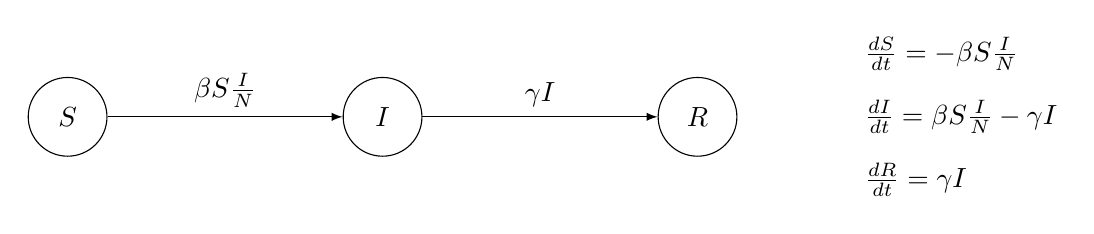
\begin{tikzpicture}
				\node[circle, draw, inner sep=0pt, minimum size=1cm] (S) at (0,0) {$S$};
				\node[circle, draw, inner sep=0pt, minimum size=1cm] (I) at (4,0) {$I$};
				\node[circle, draw, inner sep=0pt, minimum size=1cm] (R) at (8,0) {$R$};
				
				\draw[->,>=latex] (S) edge node[above] { $\beta S \frac{I}{N}$} (I);
				\draw[->,>=latex] (I) edge node[above] { $\gamma I$} (R);
				
				\node[anchor=west] at (10,.8) {$	\frac{dS}{dt} = - \beta S \frac{I}{N}$};
				\node[anchor=west] at (10,0) {$	\frac{dI}{dt} = \beta S \frac{I}{N} - \gamma I $};
				\node[anchor=west] at (10,-.8) {$\frac{dR}{dt} = \gamma I $};
			\end{tikzpicture}
		}
	\end{figure}
	Where:
	\begin{itemize}
		\item $S(t)$ is the number of people \alert{susceptible} to infection
		\item $I(t)$ is the number of people \alert{infected} (i.e. the prevalence)
		\item $R(t)$ is the number of people \alert{recovered} (lifelong immunity)
		\item $N$ is the population size ($S(t)+I(t)+R(t)=N$ for any $t$)
		\item $\beta$ is the \alert{infectious contact rate} (per day per person)
		\item $\gamma$ is the \alert{recovery rate} (1/infectious period)
	\end{itemize}
}

\frame{
	\frametitle{Introduction}
	
	\begin{figure}
		\centering
		\scalebox{.8}{
			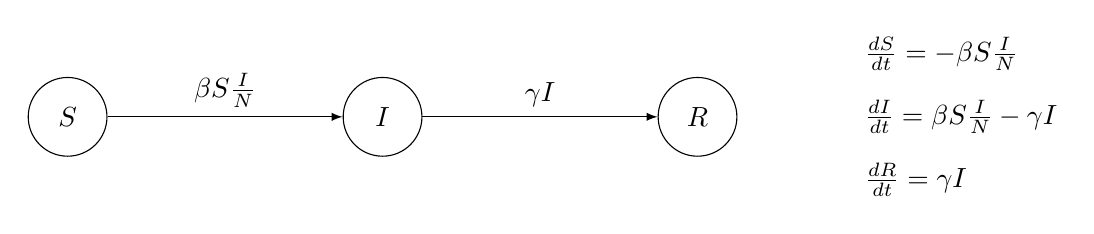
\begin{tikzpicture}
				\node[circle, draw, inner sep=0pt, minimum size=1cm] (S) at (0,0) {$S$};
				\node[circle, draw, inner sep=0pt, minimum size=1cm] (I) at (4,0) {$I$};
				\node[circle, draw, inner sep=0pt, minimum size=1cm] (R) at (8,0) {$R$};
				
				\draw[->,>=latex] (S) edge node[above] { $\beta S \frac{I}{N}$} (I);
				\draw[->,>=latex] (I) edge node[above] { $\gamma I$} (R);
				
				\node[anchor=west] at (10,.8) {$	\frac{dS}{dt} = - \beta S \frac{I}{N}$};
				\node[anchor=west] at (10,0) {$	\frac{dI}{dt} = \beta S \frac{I}{N} - \gamma I $};
				\node[anchor=west] at (10,-.8) {$\frac{dR}{dt} = \gamma I $};
			\end{tikzpicture}
		}
	\end{figure}
	\alert{Intuition} behind the SIR model:
	\begin{itemize}
		\item $I(t)/N$ is the proportion of infected (and infectious)
		\item $\beta I(t)/N$ is the daily number of contacts with infectious people
		\item hence each day, $\beta S I(t)/N$ people become infected (the \alert{force of infection})
	\end{itemize}
}

\frame{
	\frametitle{Introduction}
	
	\begin{figure}
		\centering
		\scalebox{.8}{
			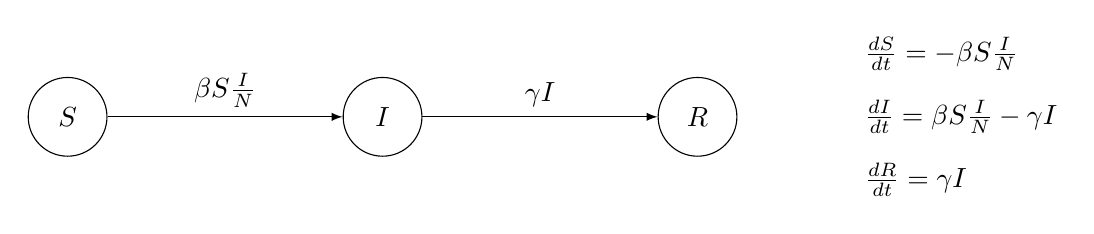
\begin{tikzpicture}
				\node[circle, draw, inner sep=0pt, minimum size=1cm] (S) at (0,0) {$S$};
				\node[circle, draw, inner sep=0pt, minimum size=1cm] (I) at (4,0) {$I$};
				\node[circle, draw, inner sep=0pt, minimum size=1cm] (R) at (8,0) {$R$};
				
				\draw[->,>=latex] (S) edge node[above] { $\beta S \frac{I}{N}$} (I);
				\draw[->,>=latex] (I) edge node[above] { $\gamma I$} (R);
				
				\node[anchor=west] at (10,.8) {$	\frac{dS}{dt} = - \beta S \frac{I}{N}$};
				\node[anchor=west] at (10,0) {$	\frac{dI}{dt} = \beta S \frac{I}{N} - \gamma I $};
				\node[anchor=west] at (10,-.8) {$\frac{dR}{dt} = \gamma I $};
			\end{tikzpicture}
		}
	\end{figure}
	\alert{Assumptions} behind the SIR model:
	\begin{itemize}
		\item homogeneous mixing
		\item $\beta$ and $\gamma$ constant over time
		\item all infections are observed
		\item no incubation, exponentially-distributed recovery
		\item lifelong immunity
		\item stable population
	\end{itemize}
}


\frame{
	\frametitle{Introduction}
	
	Simulate in \texttt{R} with package \texttt{deSolve}:
	
	\begin{itemize}
		\item set compartments and differential equations
	\end{itemize}
	\begin{figure}
		\centering
		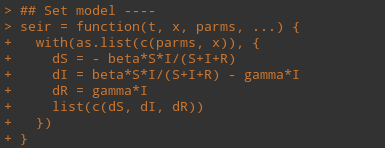
\includegraphics[width=0.55\linewidth]{simple_sir/simsir3.png}
	\end{figure}
	\pause
	\begin{itemize}
		\item set (fixed) values for 		
		$\beta=0.8$; $\rho=1/7$; $S_0=100,000-50$; $I_0=50$ and $R_0=0$
	\end{itemize}
	\begin{figure}
		\centering
		
\includegraphics[width=0.45\linewidth]{simple_sir/simsir1.png}
		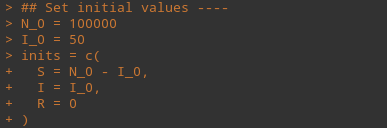
\includegraphics[width=0.45\linewidth]{simple_sir/simsir2.png}
	\end{figure}
}


\frame{
	\frametitle{Introduction}
	\begin{itemize}
		\item solve the ODE system numerically (Runge-Kutta 4th order) to obtain unique solutions for $S(t)$, $I(t)$ and $R(t)$
	\end{itemize}
	$$
f(\beta,\gamma,S_0,I_0,R_0) = \{S(t),I(t),R(t)\}
$$
	\begin{figure}
		\centering
		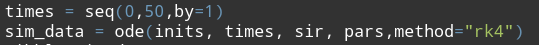
\includegraphics[width=0.65\linewidth]{simple_sir/simsir4.png}
	\end{figure}

}

\frame{
	\frametitle{Introduction}

	\begin{figure}
		\centering
		\only<1>{
			with $\beta=0.8$; $\rho=1/7$; $S_0=100000-50$; $I_0=50$ and $R_0=0$ \\ \bigskip
			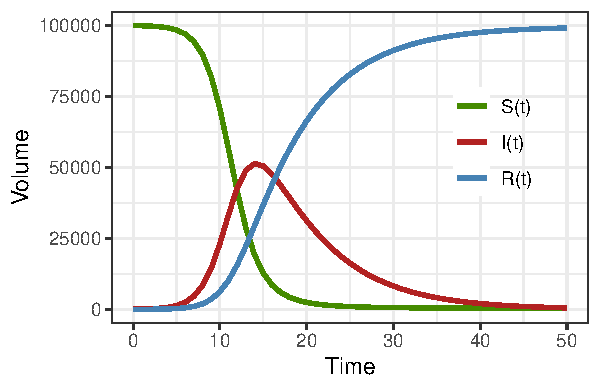
\includegraphics[width=0.7\linewidth]{simple_sir/example_sir1.pdf}
		}
		\only<2>{
			with $\beta = 1.1$ instead of $0.8$, we get \\ \bigskip
			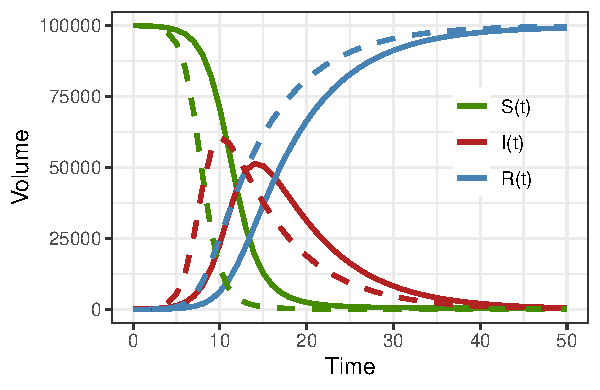
\includegraphics[width=0.7\linewidth]{simple_sir/example_sir2.pdf}
		}
		\only<3>{
			with $\beta = 0.6$ instead of $0.8$, we get \\ \bigskip
			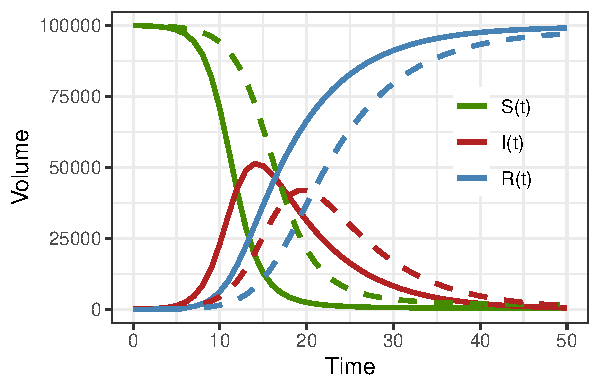
\includegraphics[width=0.7\linewidth]{simple_sir/example_sir3.pdf}
		}
		\only<4>{
		with $\gamma = 1/14$ instead of $1/7$, we get \\ \bigskip
		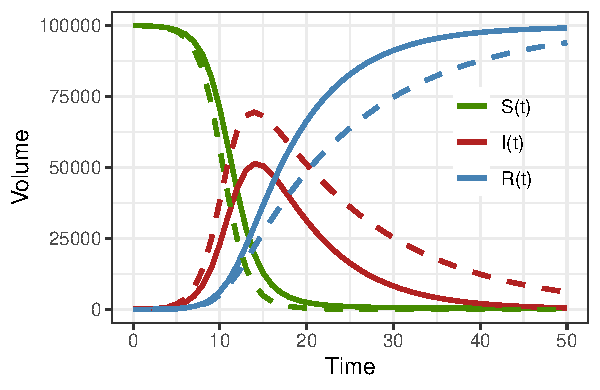
\includegraphics[width=0.7\linewidth]{simple_sir/example_sir4.pdf}
		}
		\only<5>{
		with $\gamma = 1/4$ instead of $1/7$, we get \\ \bigskip
		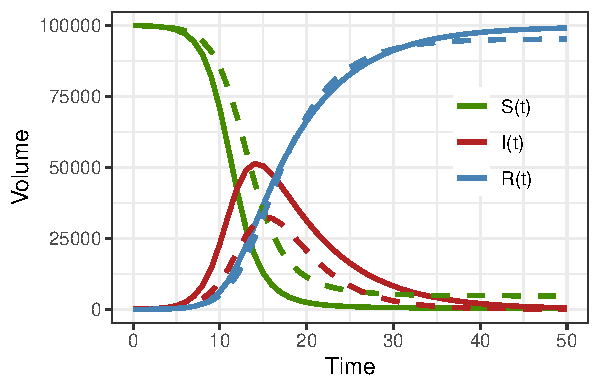
\includegraphics[width=0.7\linewidth]{simple_sir/example_sir5.pdf}
		}
		\only<6>{
		with $I(0) = 500$ instead of $50$, we get \\ \bigskip
		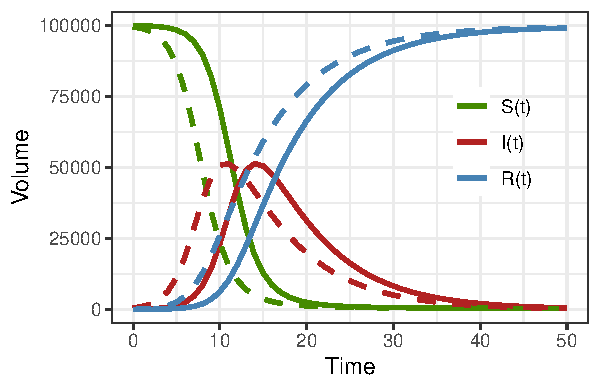
\includegraphics[width=0.7\linewidth]{simple_sir/example_sir6.pdf}
		}
		\only<7>{
		with $I(0) = 5$ instead of $50$, we get \\ \bigskip
		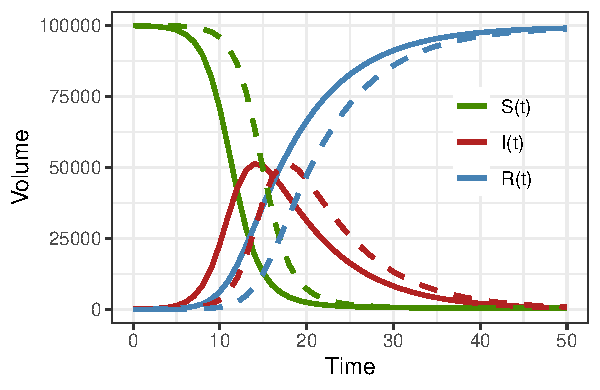
\includegraphics[width=0.7\linewidth]{simple_sir/example_sir7.pdf}
		}
		\only<8>{
		with $R(0) = 20,000$ instead of $0$, we get \\ \bigskip
		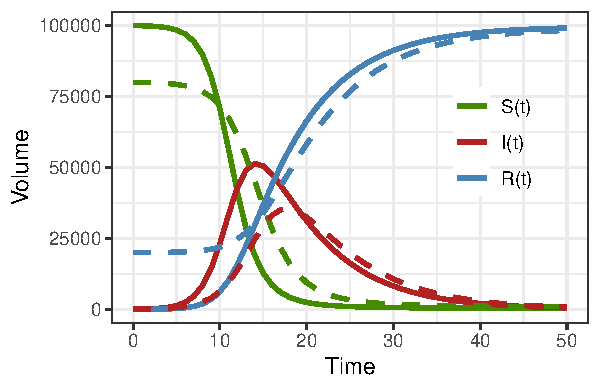
\includegraphics[width=0.7\linewidth]{simple_sir/example_sir8.pdf}
		}
	\end{figure}
}

\frame{
	\frametitle{Introduction}
	Compartmental models have many uses:
	\begin{itemize}
		\item formalize and put numerical values on \alert{general concepts} (herd immunity, vaccination threshold...)
		\item get \alert{mechanistic insight} about an epidemic (transmissibility levels, drivers of transmission)
		$$
		\mathcal{R}_0 = \frac{\beta}{\gamma}
		$$
		
		\item produce precise \alert{forecasts} (based on mechanisms)
	\end{itemize}
	
	\pause\vspace{2em}
	$\rightarrow$ all these uses are based on \alert{numerical values} for $\beta$, $\rho$ and the initial conditions and their \alert{uncertainty}
}

\frame{
	\frametitle{Introduction}
	Enters \alert{Bayesian inference}:
	\begin{itemize}
		\item infer parameter values by \alert{integrating data and domain knowledge}
		\item more efficient for complex models (high dimensionality)
		\item rigorously quantify and propagate uncertainty in parameter estimates and forecast
	\end{itemize}
	
	\pause\vspace{2em}
	$\rightarrow$ Markov Chain Monte Carlo (MCMC) methods and \alert{Stan}
}

\frame{
	\frametitle{Outline}
	\begin{itemize}
		\item Introduction
		\item \textbf{(Quick notice: Bayesian inference with Stan)}
		\item Fitting a simple SIR
		\item Simulations to understand the model
		\item Scaling up ODE-based models
		\item Extensions 
	\end{itemize}
}

\frame{
	\frametitle{(Bayesian inference with Stan)}
	General principle of Bayesian inference:
	\begin{itemize}
		\item specify a complete Bayesian model
		\begin{itemize}
			\item[-] consider data $y = \{y_1,...,y_n\}$ and parameter $\theta$
			\item[-] specify an \alert{observation model} $$\Pr(y|\theta) = \prod_n \text{normal}(y_n | \theta,1)$$
			\item[-] complete the model with a \alert{prior distribution} $$\Pr(\theta) = \text{normal}(0,1)$$
		\end{itemize}
%		\item estimate the \alert{posterior distribution of $\theta$} 
%		$$ \Pr(\theta|y) = \frac{\Pr(y|\theta) \Pr(\theta)}{\Pr(y)}  $$
		\item sample the \alert{posterior distribution} of the parameter
	\end{itemize}
}
%
%\frame{
%	\frametitle{(Bayesian inference with Stan)}
%	The \alert{joint probability density function} of the model is given by
%		$$
%		\Pr(y, \theta)
%		=
%		\prod_{n = 1}^{N} \text{normal\_pdf} \, (y_{n} \mid \theta, 1)
%		\cdot \text{normal\_pdf} \, (\theta \mid 0, 1)
%		$$
%	or on the log scale
%	$$
%	\log \Pr(y, \theta)
%	=
%	\sum_{n = 1}^{N} \text{normal\_lpdf} \, (y_{n} \mid \theta, 1)
%	+ \text{normal\_lpdf} \, (\theta \mid 0, 1) 
%	$$
%}


\frame{
	\frametitle{(Bayesian inference with Stan)}
	Stan is a probabilistic programming framework for Bayesian inference
	\begin{itemize}
		\item it is designed to let the user \alert{focus on modeling} while inference happens under the hood
		\item object-oriented language (based on \texttt{C++}) that supports many  operations, probability densities and ODE solvers
		\item extremely \alert{efficient} MCMC algorithm (Hamiltonian Monte Carlo)
		\item \alert{diagnostic tools} to evaluate the inference
		\item interfaces in \texttt{R} (package \texttt{rstan}), \texttt{python}, \texttt{julia}...	
	\end{itemize}
}



\frame{
	\frametitle{(Bayesian inference with Stan)}
	Programming in Stan is structured in \alert{blocks}:
	\begin{itemize}
		\item the \texttt{data} block defines data variables
		\begin{figure}
			\centering
			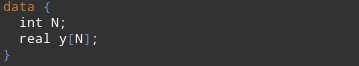
\includegraphics[width=0.6\linewidth]{example_linear/example_linear1.png}
		\end{figure}
		
		\item the \texttt{parameters} block defines parameters
		\begin{figure}
			\centering
			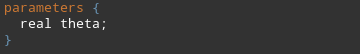
\includegraphics[width=0.6\linewidth]{example_linear/example_linear2.png}
		\end{figure}
		
		\item the \texttt{model} block defines the \alert{target log probability density function}
		\begin{figure}
			\centering
			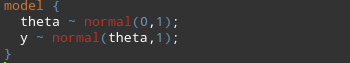
\includegraphics[width=0.6\linewidth]{example_linear/example_linear3.png}
		\end{figure}
		\item save in \texttt{model\_linear.stan}
	
	\end{itemize}
}

\frame{
	\frametitle{(Bayesian inference with Stan)}
	We then explore the target with Stan's MCMC \alert{sampler}:
	\begin{itemize}
		\item load \texttt{rstan} package
		\begin{figure}
			\centering
			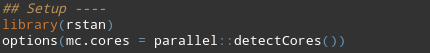
\includegraphics[width=0.7\linewidth]{example_linear/run_stan1.png}
		\end{figure}
		
		\item simulate $N=50$ data points with $\theta=0.7$
		\begin{figure}
			\centering
			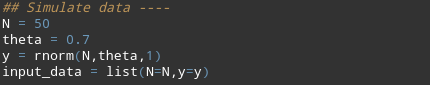
\includegraphics[width=0.7\linewidth]{example_linear/run_stan2.png}
		\end{figure}
		
		\item run MCMC sampling
		\begin{figure}
			\centering
			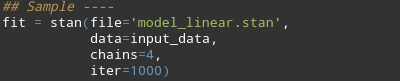
\includegraphics[width=0.7\linewidth]{example_linear/run_stan3.png}
		\end{figure}
	\end{itemize}
}

\frame{
	\frametitle{(Bayesian inference with Stan)}
	We use \alert{multiple chains} that should converge after warm-up
	\begin{figure}
		\centering
		\only<1>{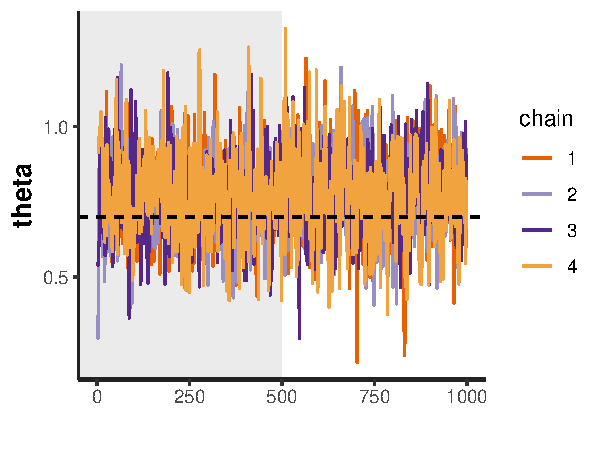
\includegraphics[width=.6\linewidth]{example_linear/trace_theta.pdf}}
		\only<2>{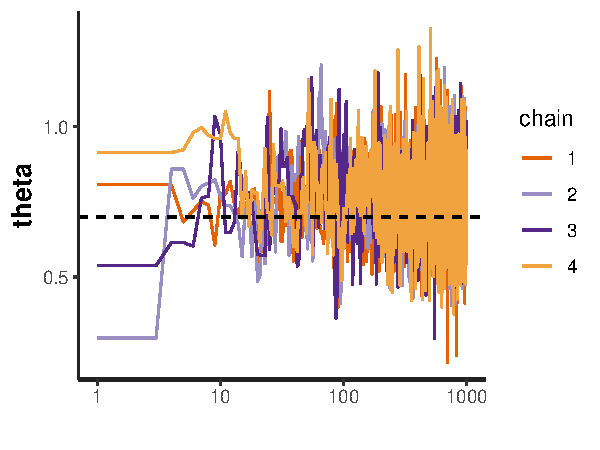
\includegraphics[width=.6\linewidth]{example_linear/trace_theta_init.pdf}}
	\end{figure}
}

\frame{
	\frametitle{(Bayesian inference with Stan)}
	The post-warm-up samples of $\theta$ approximate its \alert{posterior distribution}
	\begin{figure}
		\centering
		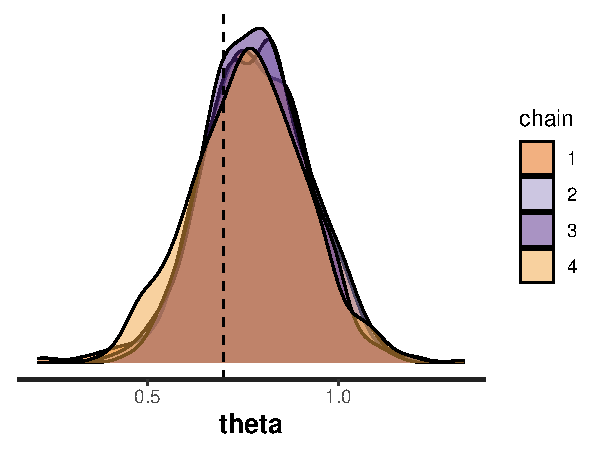
\includegraphics[width=.6\linewidth]{example_linear/post_theta.pdf}
	\end{figure}
}

\frame{
	\frametitle{(Bayesian inference with Stan)}
	
	We run \alert{basic diagnosis tools}: divergences, tree depth, energy
		\begin{figure}
			\centering
			\vspace{1em}
			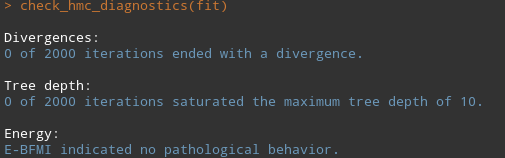
\includegraphics[width=.8\linewidth]{example_linear/run_stan5.png}
		\end{figure}

}

\frame{
	\frametitle{(Bayesian inference with Stan)}
	
	Printing the object gives:
	\begin{itemize}
		\item \alert{diagnostics}: effective sample size, Gelman-Rubin $\hat{R}$
		\item \alert{inference}: full posterior distribution of $\theta$
	\begin{figure}
		\centering
		\vspace{1em}
		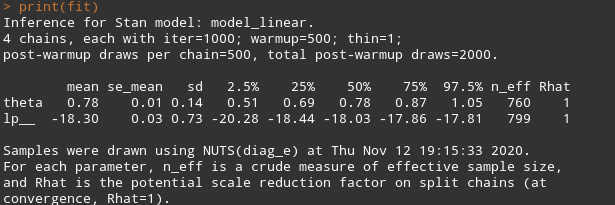
\includegraphics[width=1\linewidth]{example_linear/run_stan4.png}
	\end{figure}
	\end{itemize}
}

\frame{
	\frametitle{Outline}
	\begin{itemize}
		\item Introduction
		\item (Quick notice: Bayesian inference with Stan)
		\item \textbf{Fitting a simple SIR}
		\item Simulations to understand the model
		\item Scaling up ODE-based models
		\item Extensions 
	\end{itemize}
}

\frame{
	\frametitle{Fitting a simple SIR}
	Example data: outbreak of influenza A (H1N1) at a \alert{British boarding school} in 1978 (available in \texttt{R} package \texttt{outbreaks})
	\begin{itemize}
		\item 763 students, 512 had symptoms
		\item daily number of students in bed over 14 days (\alert{prevalence} data)
		\begin{figure}
			\centering
			\vspace{.5em}
			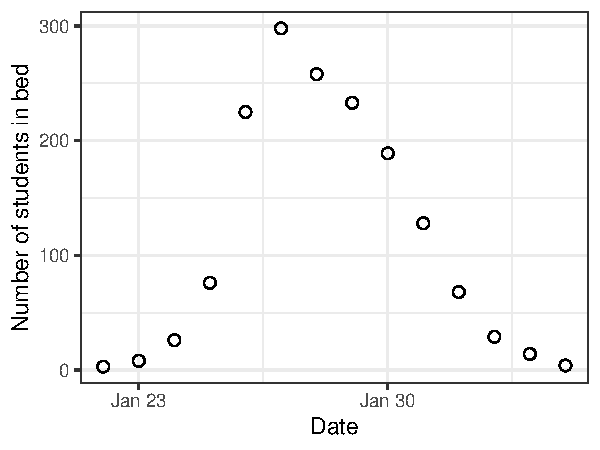
\includegraphics[width=.55\linewidth]{boarding_school/inbed.pdf}
		\end{figure}
	\end{itemize}	
}

\frame{
	\frametitle{Fitting a simple SIR}
	Specifying the model:
	\begin{itemize}
		\item prevalence data: $\mathds{I}_{t}$ with $t \in \{1,\ldots,14\}$
		\item parameters to estimate: $\theta = \{\beta,\gamma,\phi\}$
		\item parameters that will remain fixed: $\{S_0=762,I_0=1,R_0=0\}$
		\item map data $\mathds{I}_{t}$ to SIR model output $I(t)$ using an observation model  with an appropriate \alert{probability distribution}:
		$$
		\Pr(\mathds{I}|\theta) = \prod_{t=1}^{14} \text{neg-bin}(\mathds{I}_{t} | I(t), \phi)
		$$
		\item \alert{prior distributions} 
		\vspace{-1em}
		
		$$\Pr(\beta) = \text{exponential}(1)$$
		$$\Pr(1/\gamma) = \text{normal}(2,0.5)$$
		$$\Pr(1/\phi) = \text{exponential}(5)$$
	\end{itemize}
}

\frame{
	\frametitle{Fitting a simple SIR}
	We define the ODE system in the \texttt{function} block
		\begin{figure}
			\centering
			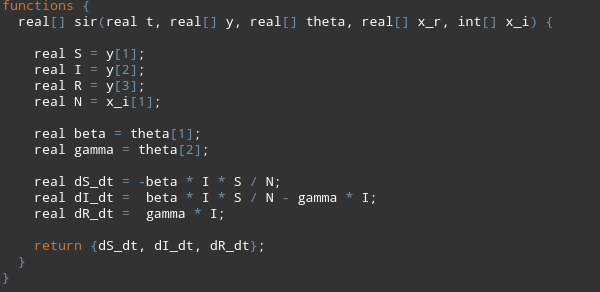
\includegraphics[width=1\linewidth]{boarding_school/stan_code1.png}
		\end{figure}
	\faWarning\ Be careful of the signature and formats!
}

\frame{
	\frametitle{Fitting a simple SIR}
	We declare the data variables in the \texttt{data} block
		\begin{figure}
			\centering
			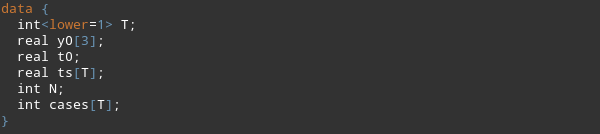
\includegraphics[width=1\linewidth]{boarding_school/stan_code2.png}
		\end{figure}
	
	\pause
	and define additional data variables in \texttt{transformed data}
	\begin{figure}
		\centering
		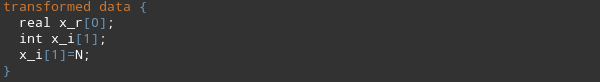
\includegraphics[width=1\linewidth]{boarding_school/stan_code3.png}
	\end{figure}
}

\frame{
	\frametitle{Fitting a simple SIR}
	Similarly, parameters are declared in the \texttt{parameters} block
		\begin{figure}
			\centering
			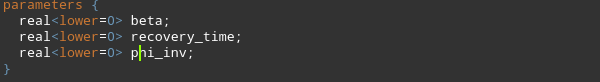
\includegraphics[width=1\linewidth]{boarding_school/stan_code4.png}
		\end{figure}
	\faWarning\ It sometimes makes more sense to transform some parameters (e.g., recovery rate $\gamma$ and overdispersion $\phi$) to improve interpretability
	}

\frame{
	\frametitle{Fitting a simple SIR}
	In \texttt{transformed parameters}, we define additional parameters and solve the ODE system
		\begin{figure}
			\centering
			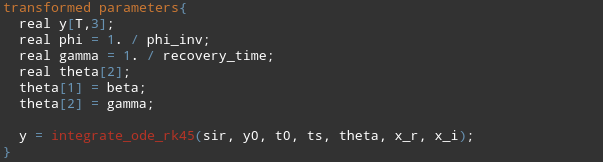
\includegraphics[width=1\linewidth]{boarding_school/stan_code5.png}
		\end{figure}
}


\frame{
	\frametitle{Fitting a simple SIR}
	\begin{figure}
		\centering
		
\includegraphics[width=.8\linewidth]{boarding_school/stan_code5bis.png}
	\end{figure}
	Two crucial points:
	\begin{itemize}
	\item be careful about the \alert{formats and signatures}
	\begin{itemize}
			\item[-] the ODE output \texttt{y} is an array of size \texttt{T}$\times$3 (number of time steps and number of compartments)
			\item[-] \texttt{sir} is the name of the function defined in the \texttt{function} block
			\item[-] \texttt{y0} is an array of size 3 defined in the \texttt{data} block
			\item[-] \texttt{ts} is an array of size \texttt{T} defined in the \texttt{data} block
			\item[-] \texttt{theta} is an array of size 2 storing the parameters
			\item[-] \texttt{x\_r} is defined as empty in \texttt{transformed data}, but can be used to store fixed real values
			\item[-] \texttt{x\_i} is an array of size 1 storing the population size \texttt{N} (can also be used to store fixed integer values)
	\end{itemize}
	\end{itemize}
}
\frame{
	\frametitle{Fitting a simple SIR}
	\begin{figure}
		\centering
		
\includegraphics[width=.8\linewidth]{boarding_school/stan_code5bis.png}
	\end{figure}
	Two crucial points:
	\begin{itemize}
		\item two ODE solvers are available:
	\begin{itemize}
		\item[-] \texttt{integrate\_ode\_rk45} uses the Runge-Kutta method (quicker but non-adapted to stiff systems)
		\item[-] \texttt{integrate\_ode\_bdf} uses the backward differentiation method (slower but adapted to stiff systems)
	\end{itemize}
	\end{itemize}
}

\frame{
	\frametitle{Fitting a simple SIR}
	In the \texttt{model} block, we write the priors and the observation model
	\begin{figure}
		\centering
		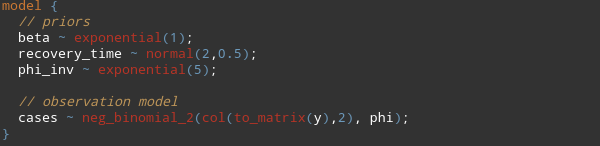
\includegraphics[width=1\linewidth]{boarding_school/stan_code6.png}
	\end{figure}
	\faWarning\ It's important that the chosen distributions correspond with the boundaries set in the \texttt{parameters} block (\texttt{<lower=0>})

\bigskip
	\faWarning\ \texttt{col(to\_to\_matrix(y))} extracts the 2nd column of \texttt{y}
}


\frame{
	\frametitle{Fitting a simple SIR}
	Last, we add a \texttt{generated quantities} block that does not influence sampling and can be used for ``post-processing'':
	\begin{itemize}
		\item reproduction number $\mathcal{R}_0 = \beta/\gamma$
		\item model predictions of prevalence from the negative binomial
	\end{itemize}

	\begin{figure}
		\centering
		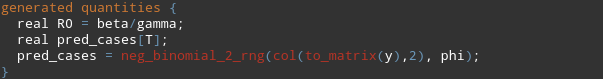
\includegraphics[width=1\linewidth]{boarding_school/stan_code7.png}
	\end{figure}
}

\frame{
	\frametitle{Fitting a simple SIR}
	In summary:
	\begin{itemize}
		\item \texttt{functions}: define the ODE system (\faWarning\ signature and formats)
		\item \texttt{data}: declare data variables that will be provided
		\item \texttt{tranformed data}: additional quantities that can be computed internally or from \texttt{data} variables 
		\item \texttt{parameters}: declare parameters (\faWarning\ boundaries)
		\item \texttt{transformed parameters}: quantities that can be computed internally or from \texttt{data} or \texttt{parameters} variables,
		including the ODE output (\faWarning \ signature and format)
		\item \texttt{model}: priors and observation model
		\item \texttt{generated quantities}: additional quantities that can be computed without influencing the sampling
	\end{itemize}

}


\frame{
	\frametitle{Fitting a simple SIR}
	As before, we conduct the inference from \texttt{R} with the package \texttt{rstan}:
	\begin{figure}
		\centering
		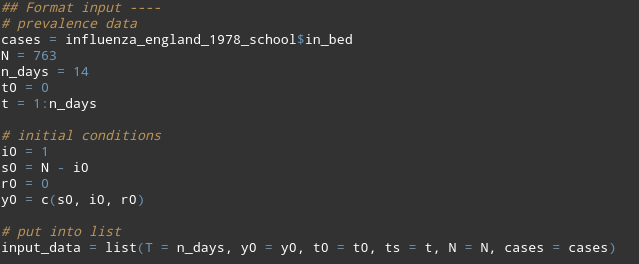
\includegraphics[width=1\linewidth]{boarding_school/r_code1.png}
	\end{figure}

	\faWarning\ data is put in a list with names matching the \texttt{data} block in Stan
}

\frame{
	\frametitle{Fitting a simple SIR}
	Hit the inference button!
	\begin{figure}
		\centering
		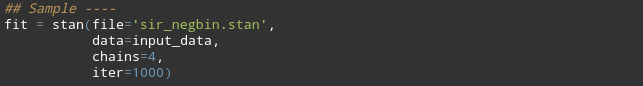
\includegraphics[width=1\linewidth]{boarding_school/r_code2.png}
	\end{figure}
}

\frame{
	\frametitle{Fitting a simple SIR}
	Run basic diagnosis tools:
	\begin{figure}
		\centering
		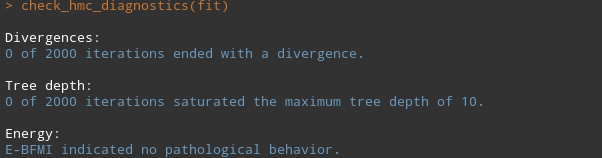
\includegraphics[width=1\linewidth]{boarding_school/r_code3.png}
	\end{figure}
}

\frame{
	\frametitle{Fitting a simple SIR}
	Examine trace plots:
	\begin{figure}
		\centering
		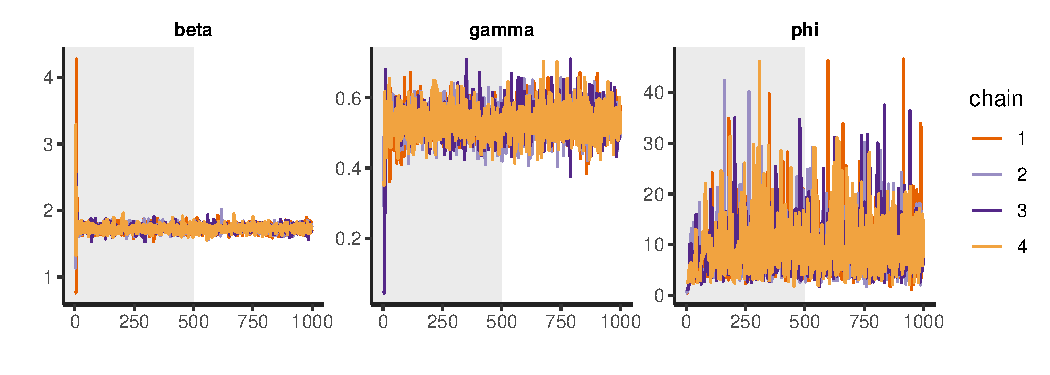
\includegraphics[width=1\linewidth]{boarding_school/trace_theta.pdf}
	\end{figure}
}

\frame{
	\frametitle{Fitting a simple SIR}
	Examine chain mixing:
	\begin{figure}
		\centering
		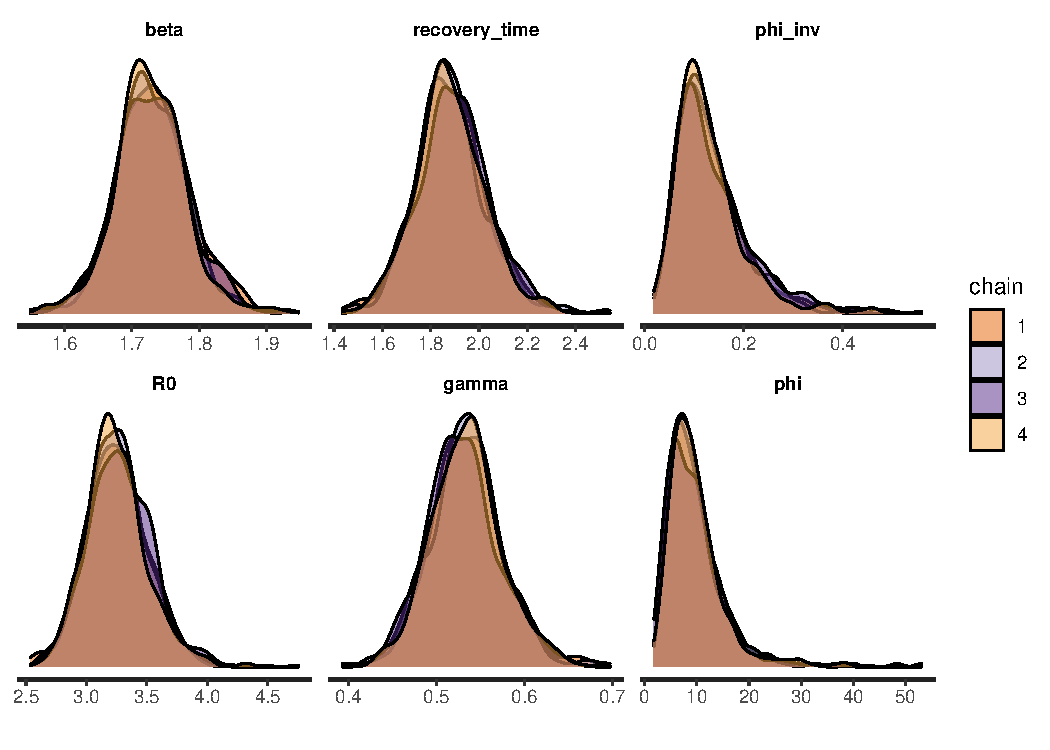
\includegraphics[width=.8\linewidth]{boarding_school/post_theta.pdf}
	\end{figure}
}

\frame{
	\frametitle{Fitting a simple SIR}
	Posterior predictive checking (always show!):
	\begin{figure}
		\centering
		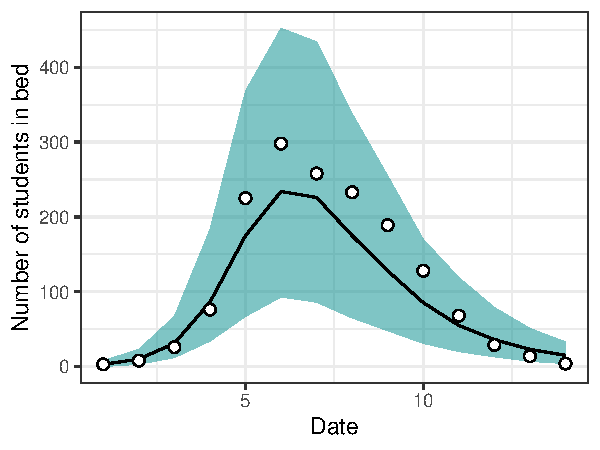
\includegraphics[width=.6\linewidth]{boarding_school/inbed_fit.pdf}
	\end{figure}
}

\frame{
	\frametitle{Fitting a simple SIR}
	Print the results:
	\begin{figure}
		\centering
		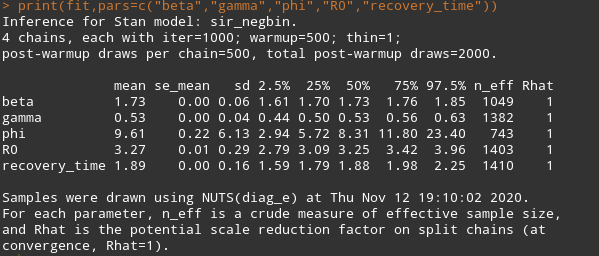
\includegraphics[width=1\linewidth]{boarding_school/r_code4.png}
	\end{figure}
}

\frame{
	\frametitle{Fitting a simple SIR}
	Conclusions:
	\begin{itemize}
		\item we estimate $\mathcal{R}_0$ to 3.3 (95\% credible interval: 2.8 to 4.0)
		\item this corresponds to the direct estimation from the final size of the epidemic $q = 512/763 = 0.67$
		\vspace{-.5em}
		$$
		\mathcal{R}_0 = 1 / (1-q) = 3.03
		$$
		\item based on \alert{many assumptions}:
		\begin{itemize}
			\item[-] common to all SIRs (homogeneous mixing, no incubation...)
			\item[-] prior distributions (especially on the recovery period)
			\item[-] complete ascertainment, no asymptomatics
			\item[-] no initial immunity
		\end{itemize}
	\end{itemize}
		
}

\frame{
	\frametitle{Outline}
	\begin{itemize}
		\item Introduction
		\item (Quick notice: Bayesian inference with Stan)
		\item Fitting a simple SIR
		\item \textbf{Simulations to understand the model}
		\item Scaling up ODE-based models
		\item Extensions 
	\end{itemize}
}

\frame{
	\frametitle{Simulations to understand the model}
	In practice, the situation is often less clear than in the boarding school example:
	\begin{itemize}
		\item[-] incomplete data, insufficient domain knowledge
		\item[-] uncertainty on \alert{necessary model features}
	\end{itemize}
	\alert{Fake data} can be used to probe the model and better understand its behaviour:
	\begin{itemize}
		\item[-] prior predictive checking
		\item[-] simulation study
	\end{itemize}	
}

\frame{
	\frametitle{Simulations to understand the model}
	\alert{Prior predictive checking} consists in simulating data from the priors:
	\begin{itemize}
		\item visualize priors (especially after transformation)
		\item this shows the range of data compatible with the model
		\item it helps understand the \alert{adequacy of the chosen priors}, as it is often easier to elicit expert knowledge on measureable quantities of interest rather than abstract parameter values
		\bigskip\pause
		\item remove (or switch off) the likelihood from the \texttt{model} block
	\end{itemize}
	\begin{figure}
		\centering
		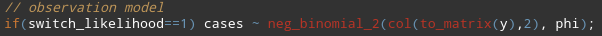
\includegraphics[width=1\linewidth]{boarding_school/stan_code6bis.png}
	\end{figure}
}

\frame{
	\frametitle{Simulations to understand the model}
	Simulating priors in the boarding school example:
	\begin{figure}
		\centering
		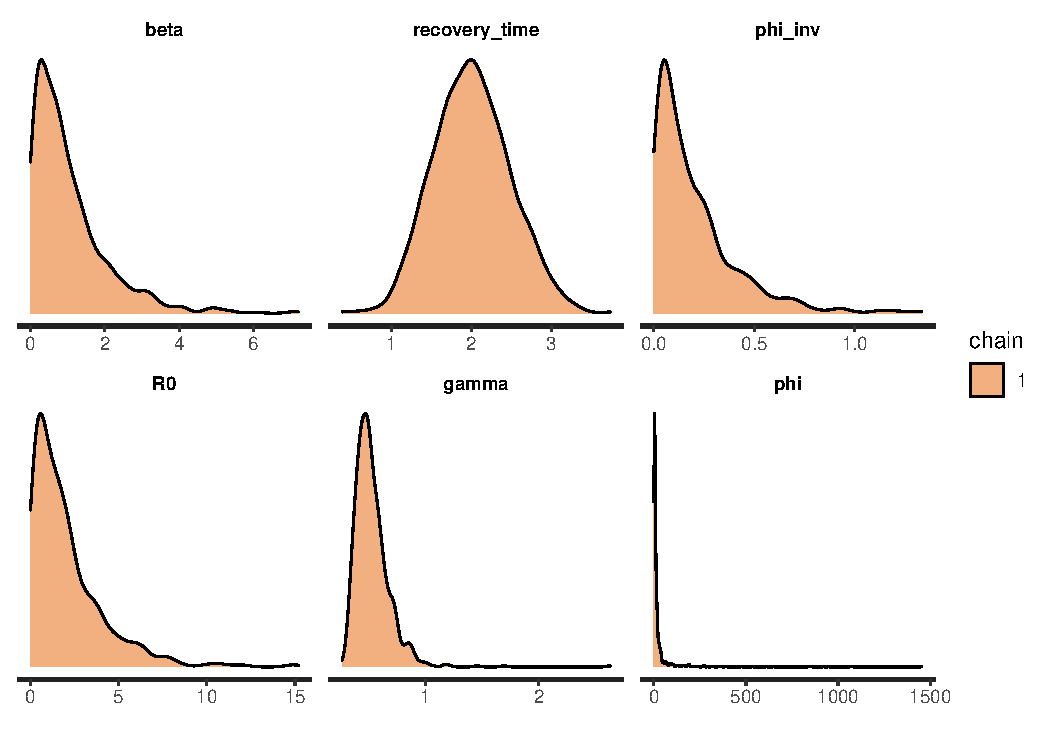
\includegraphics[width=.8\linewidth]{boarding_school/prior_theta.pdf}
	\end{figure}
}

\frame{
	\frametitle{Simulations to understand the model}
	Prior predictive checking: simulating \alert{epidemic trajectories}
	\begin{figure}
		\centering
		\only<1>{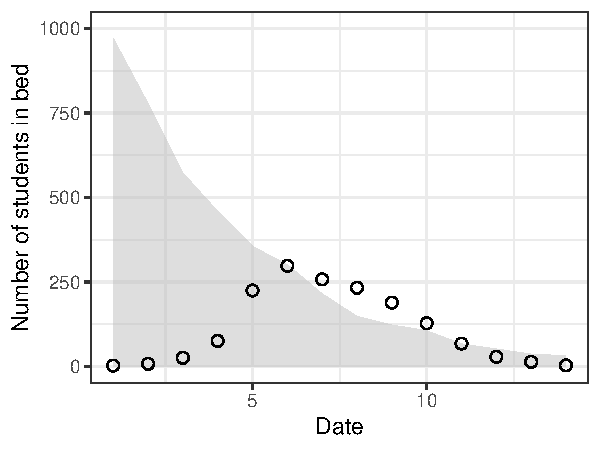
\includegraphics[width=.6\linewidth]{boarding_school/inbed_fit_prior.pdf}}
		\only<2>{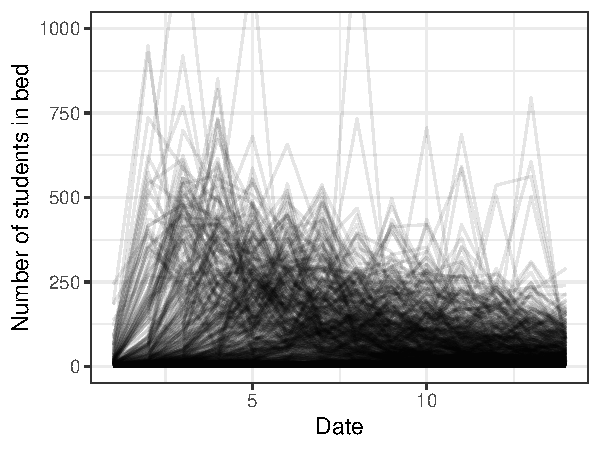
\includegraphics[width=.6\linewidth]{boarding_school/inbed_fit_prior_traj.pdf}}
	\end{figure}
}

\frame{
	\frametitle{Simulations to understand the model}
	Prior predictive checking brings insight about \alert{non-obvious features}:
	\begin{itemize}
		\item even if the priors seem weakly informative, there is actually not a lot of leeway
		\item \alert{highly constrained} model: 
		\begin{itemize}
		\item[-] if $\beta$ is high, the epidemic will stop rapidly by lack of susceptibles
		\item[-] if $\beta$ is small, the epidemic will be small
	\end{itemize}
	\item the negative binomial might lead to problems in extreme situations, e.g. more cases (>1000) than the overall number of students
	\end{itemize}
}

\frame{
	\frametitle{Simulations to understand the model}
	A \alert{simulation study} consists in two steps:
	\begin{itemize}
		\item simulate data with specified parameter values
		\item measure the capacity of the model to recover the chosen parameter values
\end{itemize}
	\bigskip\pause
	Many advantages:
	\begin{itemize}
	\item check for bugs and coding mistakes
	\item check for \alert{identifiability} issues
	\item compare different versions of a model
	\item understand in what \alert{situations} a model works or not
\end{itemize}
}

\frame{
	\frametitle{Simulations to understand the model}
	Let's go back to the \alert{simple SIR example} from the beginning:
	\begin{itemize}
		\item set $\beta=2$ and $\gamma=0.5$ (so that $\mathcal{R}_0=4$) 
		\item simulate in a susceptible population of size $N=763$ with $I_0=1$
	\end{itemize}
	\begin{figure}
	\centering
	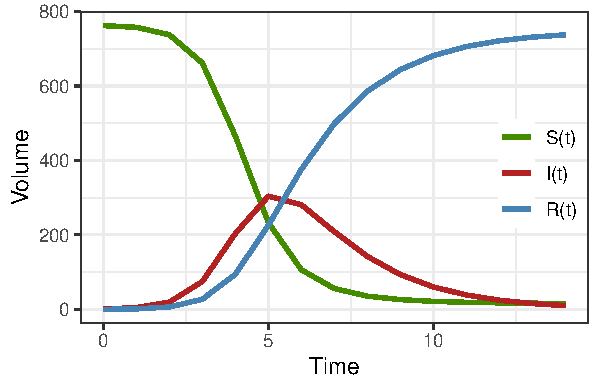
\includegraphics[width=.6\linewidth]{boarding_school/example_sir1.pdf}
\end{figure}
}

\frame{
	\frametitle{Simulations to understand the model}
	Add noise with a \alert{negative binomial} distribution with $\phi=15$
	\begin{figure}
		\centering
		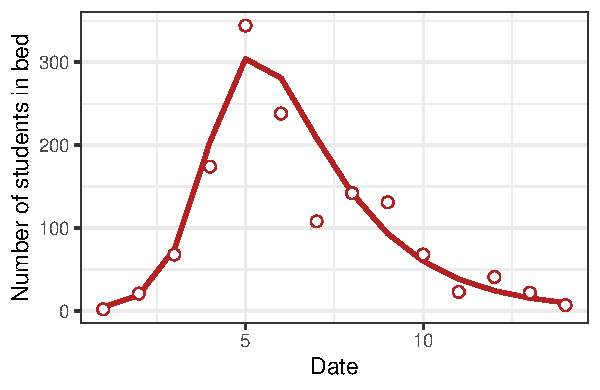
\includegraphics[width=.6\linewidth]{boarding_school/example_sir2.pdf}
	\end{figure}
}

\frame{
	\frametitle{Simulations to understand the model}
	Fit the \alert{same model} as for the boarding school example
	\begin{figure}
		\centering
		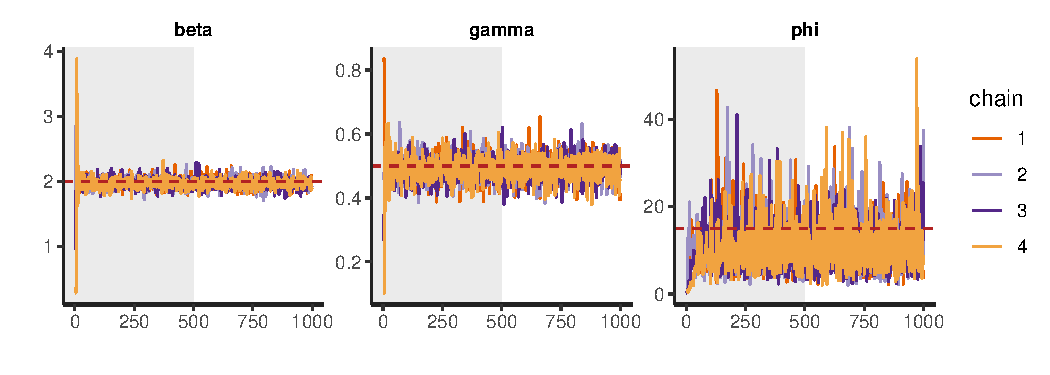
\includegraphics[width=1\linewidth]{boarding_school/trace_theta_sim.pdf}
	\end{figure}
}


\frame{
	\frametitle{Simulations to understand the model}
	Posterior predictive checking
	\begin{figure}
		\centering
		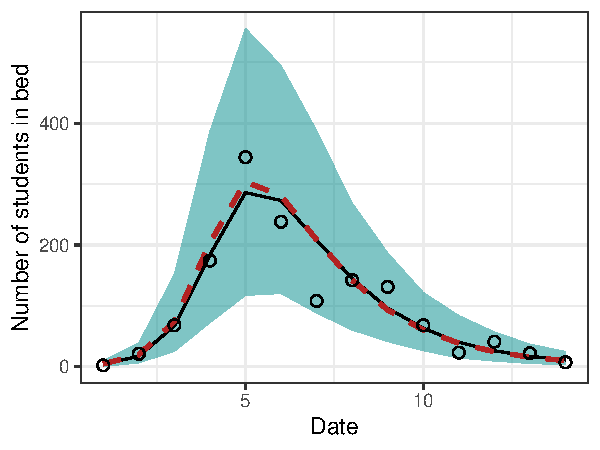
\includegraphics[width=.6\linewidth]{boarding_school/inbed_fit_sim.pdf}
	\end{figure}
}


\frame{
	\frametitle{Simulations to understand the model}
	\bigskip
	Compare the posterior distributions of the parameters with the \alert{``truth''}
	\begin{figure}
		\centering
		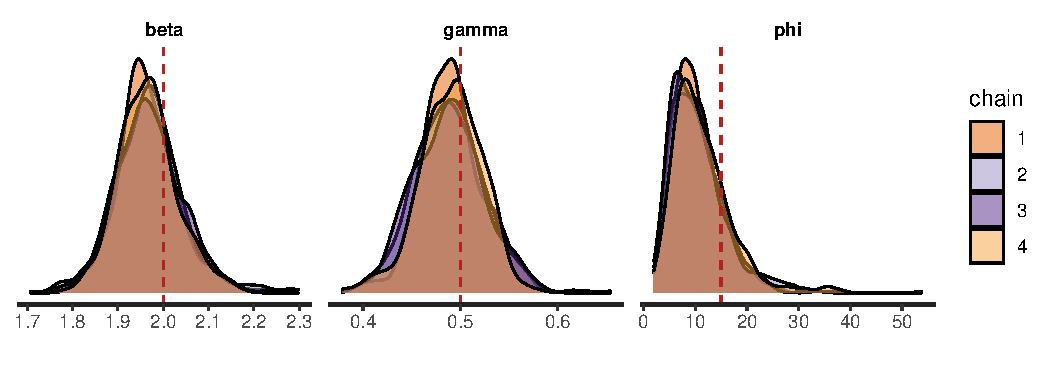
\includegraphics[width=.9\linewidth]{boarding_school/post_theta_sim.pdf}
	\end{figure}
	\begin{itemize}
		\vspace{-1em}
	\item no identifiability issue
	\item $\beta$ and $\gamma$ are well estimated, but $\phi$ is not
	\item try with other values to understand \alert{when does the model break}
	\end{itemize}
}

\frame{
	\frametitle{Outline}
	\begin{itemize}
		\item Introduction
		\item (Quick notice: Bayesian inference with Stan)
		\item Fitting a simple SIR
		\item {Simulations to understand the model}
		\item \textbf{Scaling up ODE-based models}
		\item Extensions 
	\end{itemize}
}

\frame{
	\frametitle{Scaling up ODE-based models}
	Inference with ODE-based models is \alert{computationally intensive}
	\bigskip
	
	Be attentive to the model structure:
		\begin{itemize}
		\item HMC requires to compute the \alert{gradient} of the log joint density 
		multiple times for each iteration 
		$$
		\triangledown_{\theta}\log \Pr(y,\theta)
		$$
		 \item each block is treated differently
		 	\begin{itemize}
		 	\item[-] \texttt{transformed data} and \texttt{generated quantities} are evaluated once per iteration
		 	\item[-] \texttt{parameters}, \texttt{transformed parameters} and \texttt{model} are evaluated multiple times for each iteration
		 	\item[$\rightarrow$] put everything that \alert{does not influence the inference} (e.g. $\mathcal{R}_0$ or predicted values)  in \texttt{generated quantities} 
	 			 \end{itemize}
	\end{itemize}
		
}


\frame{
	\frametitle{Scaling up ODE-based models}
	\alert{Limiting the load} of the ODE solver:
	\begin{figure}
		\centering
		
\includegraphics[width=.8\linewidth]{boarding_school/stan_code5bis.png}
	\end{figure}
	\begin{itemize}
		\item the computational cost of solving the ODEs scales with $N + NK$
		\begin{itemize}
			\item[-] $N$: the number of compartments
			\item[-] $K$: the number of parameters in \texttt{y0} and \texttt{theta}
		\end{itemize}
		\item[$\rightarrow$] remove unnecessary compartments (e.g. $R(t)$)
		\item[$\rightarrow$] reparametrize initial conditions
	\end{itemize}
	
}

\frame{
	\frametitle{Scaling up ODE-based models}
	Picking \alert{the right ODE solver}:
	\begin{itemize}
		\item two are available:
	\begin{itemize}
		\item[-] \texttt{integrate\_ode\_rk45} uses the Runge-Kutta method (quicker but non-adapted to stiff systems)
		\item[-] \texttt{integrate\_ode\_bdf} uses the backward differentiation method (slower but adapted to stiff systems)
	\end{itemize}
	\item there is no formal definition of \alert{stiffness}
	\item intuitively, it occurs when the time step of the integrator needs to be very small to keep the solution stable (e.g. large variations in magnitude in time)
	\item[$\rightarrow$] start with \texttt{rk45}, move to \texttt{bdf} if there are problems (\textit{folk theorem of statistical computing})
\end{itemize}
}

\frame{
	\frametitle{Scaling up ODE-based models}
	\alert{Tuning} the ODE solver:
		\begin{itemize}
		\item additional options in the solver function
		\begin{figure}
		\centering
		\includegraphics[width=.8\linewidth]{boarding_school/tolerances.png}
	\end{figure}
		\begin{itemize}
			\item[-] \texttt{rel\_tol} is the relative tolerance
			\item[-] \texttt{abs\_tol} is the absolute tolerance
			\item[-] \texttt{max\_steps} is the maximum number of steps 
		\end{itemize}
	\item can be adjusted depending on the level of \alert{precision} needed
	\end{itemize}

	\bigskip
	\faWarning\ be cause of the tolerance, the ODE solver may sometimes give negative values when too close to zero, causing issues
	
	\vspace{.2em}$\rightarrow$ this can be solved by \alert{adding 5-10 times the absolute tolerance} to the ODE output
}

\frame{
	\frametitle{Outline}
	\begin{itemize}
		\item Introduction
		\item (Quick notice: Bayesian inference with Stan)
		\item Fitting a simple SIR
		\item {Simulations to understand the model}
		\item {Scaling up ODE-based models}
		\item \textbf{Extensions} 
	\end{itemize}
}

\frame{
	\frametitle{Extensions}
	In practice, the boarding school example quickly reaches its \alert{limits}:
	\begin{itemize}
		\item epidemics are not often observed in such a controlled environment (\alert{under-ascertainment})
		\item epidemics are not always left uncontrolled
		\item data generally consist of daily counts of new cases (\alert{incidence}) rather than counts of currently sick people (\alert{prevalence})
		\item most infectious diseases have an \alert{incubation period} (SEIR instead of SIR)
		\item transmission is generally not homogeneous in the full population (\alert{stratification} by age, sex...)
		\item ...
	\end{itemize}
}

\frame{
	\frametitle{Extensions}
	Example with SARS-CoV-2 from \alert{Hauser et al.~(2020)}:
	\vspace{1em}
	
	\begin{figure}
		\centering
		\includegraphics[width=.9\linewidth]{example_hauser/paper_ref.png}
	\end{figure}
}

\frame{
	\frametitle{Background}
	The \alert{case fatality ratio} (CFR) is computed as the number of deaths divided by the number of reported cases at time $t$.
	\bigskip
	
	Estimated in real time, the CFR is a misleading indicator of mortality due to SARS-CoV-2 because of two opposing biases:
	\begin{itemize}
		\item \alert{preferential ascertainment of severe cases}: severe cases are both more likely to die and more likely to be diagnosed and reported
		\item[$\rightarrow$] overestimates mortality
		\vspace{.4em}
		\item \alert{right-censoring} of deaths: there is a long delay between infection and deaths, so that part of the cases at time $t$ will die in the future
		\item[$\rightarrow$] underestimates mortality
	\end{itemize}
}

\frame{
	\frametitle{Background}
	This \alert{limits the interpretability} of the CFR:
	
	\begin{itemize}
		\item varies in time (ascending or descending phase)
		\item varies across countries (depending on surveillance system)
		
		\item[$\rightarrow$] April 2020: from 2.4\% in Wuhan to 17.8\% in Lombardy)
		
		\bigskip
		\item the real indicator of interest is the \alert{infection fatality ratio}, i.e. the total number of deaths that occur among people infected with SARS-CoV-2
	\end{itemize}
}

\frame{
	\frametitle{Objectives}
	\begin{itemize}
		\item[(1)] Simulate the dynamics of transmission and mortality of SARS-CoV-2 using publicly available surveillance data 
		
		\item[(2)] Provide \alert{overall and age-stratified estimates of IFR} for SARS-CoV-2 infection adjusted for right-censoring and preferential ascertainment
		
		\bigskip
		 in \alert{seven different geographic locations} with available data on:
		 \item reported cases by date of disease onset
		 \item deaths linked to SARS-CoV-2 infection by date of death
		 \item age distribution of cases
		 \item age distribution of deaths
	\end{itemize}
}


\frame{
	\frametitle{Data}
	In Hubei province (China):
	\begin{figure}
		\centering
				\includegraphics[width=.9\linewidth]{example_hauser/data_china.pdf}
	\end{figure}
}


\frame{
	\frametitle{Model development}
	Specific features and natural history of SARS-CoV-2 infection:
	\begin{itemize}
		\item Incubation period of 5 days (S\alert{E}IR)
		\item Pre-symptomatic transmission accounting for 44-48\% (SE\alert{P}IR)
		\item Symptoms in 81\% (95\%CrI 71\%–89\%) of cases (SEPI\alert{A}R)
		\item Respiratory virus transmitted through contacts (\alert{age stratification})
		\item Effect of control measures (\alert{time-dependent force of infection})
		\item Mortality is delayed by $20.2 \pm 11.6$ days (\alert{fit to mortality data})
	\end{itemize}
}

\frame{
	\frametitle{Model development}
	 Final model:
	 \begin{figure}
	 \scalebox{.8}{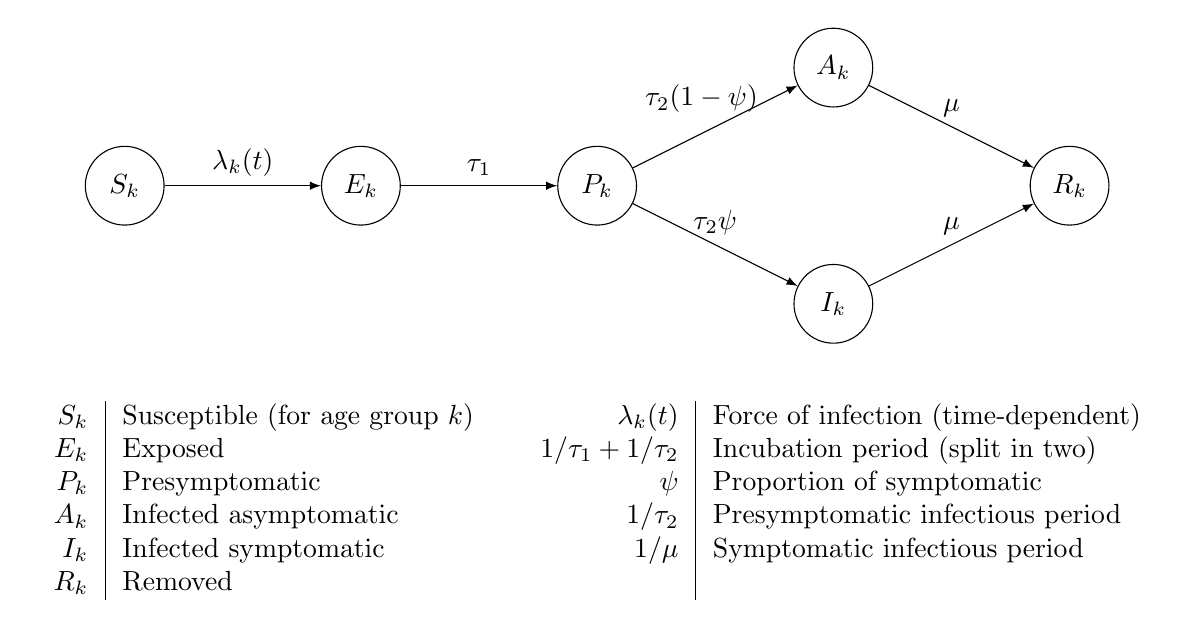
\begin{tikzpicture}
	 		% cascade of care
	 		\node[circle, draw, inner sep=0pt, minimum size=1cm] (S) at (0,0) {$S_k$};
	 		\node[circle, draw, inner sep=0pt, minimum size=1cm] (E) at (3,0) {$E_k$};
	 		\node[circle, draw, inner sep=0pt, minimum size=1cm] (P) at (6,0) {$P_k$};
%	 		\node[circle, draw, inner sep=0pt, minimum size=1cm,gray,dashed] (C) at (8.5,-2.5) {$C_k$};
%	 		\node[circle, draw, inner sep=0pt, minimum size=1cm,gray,dashed] (rho_C) at (12,-2.5) {$\rho_k C_k$};
	 		\node[circle, draw, inner sep=0pt, minimum size=1cm,fill=white] (I) at (9,-1.5) {$I_k$};
	 		\node[circle, draw, inner sep=0pt, minimum size=1cm] (A) at (9,1.5) {$A_k$};
	 		\node[circle, draw, inner sep=0pt, minimum size=1cm] (R) at (12,0) {$R_k$};
	 		
	 		\draw[->,>=latex] (S) edge node[above] { $\lambda_k(t)$} (E);
	 		\draw[->,>=latex] (E) edge node[above] { $\tau_1$ } (P);
	 		\draw[->,>=latex] (P) edge node[yshift=10,xshift=-5] { $\tau_2(1-\psi)$ } (A);
	 		\draw[->,>=latex] (P) edge node[above] { $\tau_2\psi$ } (I);
%	 		\draw[->,>=latex,gray,dashed] (P) edge[bend left=12] node[below] { $\tau_2\psi$ } (C);
	 		\draw[->,>=latex] (A) edge node[above] { $\mu$ } (R);
	 		\draw[->,>=latex] (I) edge node[above] { $\mu$ } (R);
%	 		\draw[double,gray] (C) -- node[above] { $\rho_k$ }  (rho_C);
%	 		
%	 		% legend
	 		\node (leg) at (6,-4) {
	 			\begin{tabular}{r|lp{0cm}r|l}
	 				$S_k$ & Susceptible (\alert{for age group $k$})& & $\lambda_k(t)$ & Force of infection (\alert{time-dependent})\\
	 				$E_k$ & Exposed & & $1/\tau_1+1/\tau_2$ & Incubation period (\alert{split in two})\\
	 				$P_k$ & Presymptomatic & &$\psi$ & Proportion of symptomatic \\	
	 				$A_k$ & Infected asymptomatic & & 	$1/\tau_2$ & Presymptomatic infectious period \\
	 				$I_k$ & Infected symptomatic& &	 $1/\mu$ & Symptomatic infectious period \\
	 				$R_k$ & Removed & & &\\% $\rho_k$ & Ascertainment proportion \\
	 			%	$C_k$ & Cumulative cases  & & $\rho_k C_k$ & Cumulative confirmed cases \\
	 		\end{tabular}};
	 	\end{tikzpicture}
 	}
 \end{figure}
}



\frame{
	\frametitle{Model development}
	\alert{Incubation}:
	\begin{itemize}
		\item \alert{SEIR}: adding a compartment \alert{$E$ for exposed}, i.e. infected but not yet symptomatic

	\bigskip
	\begin{figure}
		\scalebox{.8}{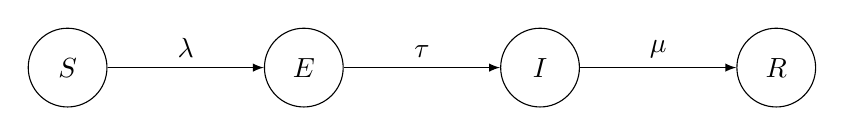
\begin{tikzpicture}
				% cascade of care
				\node[circle, draw, inner sep=0pt, minimum size=1cm] (S) at (0,0) {$S$};
				\node[circle, draw, inner sep=0pt, minimum size=1cm] (E) at (3,0) {$E$};
				\node[circle, draw, inner sep=0pt, minimum size=1cm] (I) at (6,0) {$I$};
				\node[circle, draw, inner sep=0pt, minimum size=1cm] (R) at (9,0) {$R$};
				
				\draw[->,>=latex] (S) edge node[above] { $\lambda$} (E);
				\draw[->,>=latex] (E) edge node[above] { $\tau$ } (I);
				\draw[->,>=latex] (I) edge node[above] { $\mu$ } (R);
			\end{tikzpicture}}
		
		\bigskip
	\end{figure}
	\begin{itemize}
	\item[-] $\tau$ is the inverse of the incubation period
	\bigskip
	\item[-] \alert{individuals are infectious from symptom onset} (when entering $I$)
	$$
	\lambda = \beta \frac{I}{N}
	$$
	\end{itemize}
	\end{itemize}


}

\frame{
	\frametitle{Model development}
	\bigskip
	\alert{Pre-symptomatic transmission}:
	\begin{itemize}
		\item \alert{SEPIR}: adding a compartment \alert{P for pre-symptomatic}, i.e. not yet symptomatic but already infectious
		\bigskip
	\begin{figure}
		\scalebox{.8}{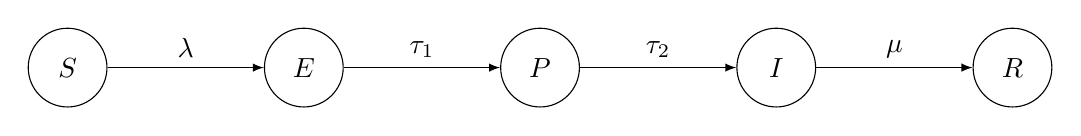
\begin{tikzpicture}
				% cascade of care
				\node[circle, draw, inner sep=0pt, minimum size=1cm] (S) at (0,0) {$S$};
				\node[circle, draw, inner sep=0pt, minimum size=1cm] (E) at (3,0) {$E$};
				\node[circle, draw, inner sep=0pt, minimum size=1cm] (P) at (6,0) {$P$};
				\node[circle, draw, inner sep=0pt, minimum size=1cm] (I) at (9,0) {$I$};
				\node[circle, draw, inner sep=0pt, minimum size=1cm] (R) at (12,0) {$R$};
				
				\draw[->,>=latex] (S) edge node[above] { $\lambda$} (E);
				\draw[->,>=latex] (E) edge node[above] { $\tau_1$ } (P);
				\draw[->,>=latex] (P) edge node[above] { $\tau_2$ } (I);
				\draw[->,>=latex] (I) edge node[above] { $\mu$ } (R);
		\end{tikzpicture}}
		
		\bigskip
	\end{figure}
	\begin{itemize}
		\item[-] the incubation period is split in two phases with rates $\tau_1$ and $\tau_2$
		\item[-] individuals are infectious \alert{before symptom onset} (entering $P$)
		$$
		\lambda = \beta \frac{P+I}{N}
		$$
		\item[-] we can introduce \alert{reduced transmissibility} before symptom onset
		$$
		\lambda = \beta \frac{\kappa P+I}{N}
		$$
	\end{itemize}
\end{itemize}	
}

\frame{
	\frametitle{Model development}
	\bigskip
	\alert{Asymptomatic} infections:
	\begin{itemize}
		\item \alert{SEPIAR}: adding a compartment \alert{A for asymptomatic}
		\bigskip
		\begin{figure}
			\scalebox{.8}{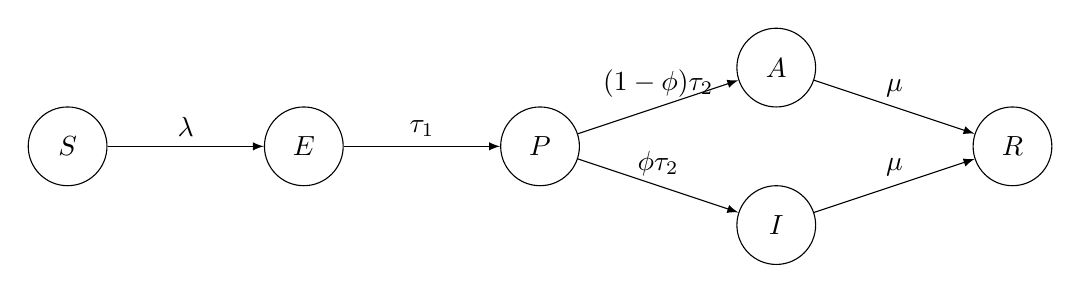
\begin{tikzpicture}
					% cascade of care
					\node[circle, draw, inner sep=0pt, minimum size=1cm] (S) at (0,0) {$S$};
					\node[circle, draw, inner sep=0pt, minimum size=1cm] (E) at (3,0) {$E$};
					\node[circle, draw, inner sep=0pt, minimum size=1cm] (P) at (6,0) {$P$};
					\node[circle, draw, inner sep=0pt, minimum size=1cm] (A) at (9,1) {$A$};
					\node[circle, draw, inner sep=0pt, minimum size=1cm] (I) at (9,-1) {$I$};
					\node[circle, draw, inner sep=0pt, minimum size=1cm] (R) at (12,0) {$R$};
					
					\draw[->,>=latex] (S) edge node[above] { $\lambda$} (E);
					\draw[->,>=latex] (E) edge node[above] { $\tau_1$ } (P);
					\draw[->,>=latex] (P) edge node[above] { $\phi\tau_2$ } (I);
					\draw[->,>=latex] (P) edge node[above] { $(1-\phi)\tau_2$ } (A);
					\draw[->,>=latex] (I) edge node[above] { $\mu$ } (R);
					\draw[->,>=latex] (A) edge node[above] { $\mu$ } (R);
			\end{tikzpicture}}
			
			\bigskip
		\end{figure}
		\begin{itemize}
			\item[-] we introduce the proportion of symptomatics $\phi$

			\item[-] we can introduce \alert{reduced transmissibility} for asymptomatics
			$$
			\lambda = \beta \frac{\kappa P+I+ \kappa A}{N}
			$$
		\end{itemize}
	\end{itemize}	
}


\frame{
	\frametitle{Model development}
	\alert{Age stratification}:
	\begin{itemize}
		\item the \alert{transmission} of respiratory viruses (influenza virus, rhinovirus...) is {highly dependent on age} 
		\item the \alert{mortality} of respiratory infections (even more so for SARS-CoV-2) is highly dependent on age
		\bigskip
		\item[$\rightarrow$] stratification in nine age groups $k\in\{1,\ldots,9\}$ for (0-9, \ldots, 80+)
		\end{itemize}
	\begin{figure}
	\scalebox{.8}{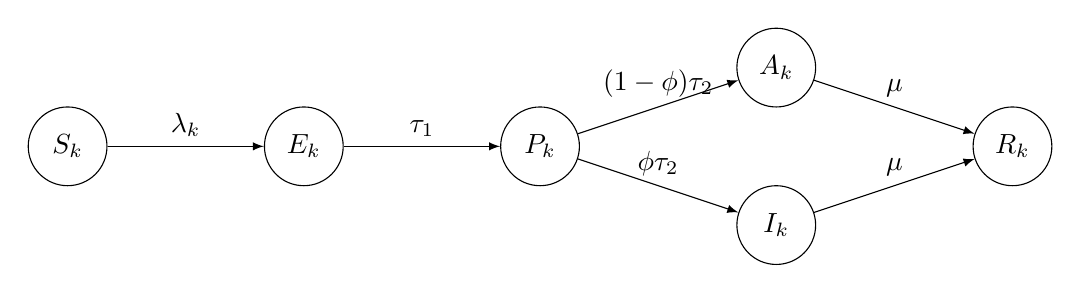
\begin{tikzpicture}
			% cascade of care
			\node[circle, draw, inner sep=0pt, minimum size=1cm] (S) at (0,0) {$S_k$};
			\node[circle, draw, inner sep=0pt, minimum size=1cm] (E) at (3,0) {$E_k$};
			\node[circle, draw, inner sep=0pt, minimum size=1cm] (P) at (6,0) {$P_k$};
			\node[circle, draw, inner sep=0pt, minimum size=1cm] (A) at (9,1) {$A_k$};
			\node[circle, draw, inner sep=0pt, minimum size=1cm] (I) at (9,-1) {$I_k$};
			\node[circle, draw, inner sep=0pt, minimum size=1cm] (R) at (12,0) {$R_k$};
			
			\draw[->,>=latex] (S) edge node[above] { $\lambda_k$} (E);
			\draw[->,>=latex] (E) edge node[above] { $\tau_1$ } (P);
			\draw[->,>=latex] (P) edge node[above] { $\phi\tau_2$ } (I);
			\draw[->,>=latex] (P) edge node[above] { $(1-\phi)\tau_2$ } (A);
			\draw[->,>=latex] (I) edge node[above] { $\mu$ } (R);
			\draw[->,>=latex] (A) edge node[above] { $\mu$ } (R);
	\end{tikzpicture}}

	\end{figure}
}

\frame{
	\frametitle{Model development}
	Characterizing the \alert{force of infection}:
	\begin{itemize}
		\item in the simple SIR, the force of infection is defined as the rate at which susceptible individuals acquire infection
		$$
		\lambda = \beta \frac{I}{N}
		$$
		
		\item the transmission rate $\beta$ can be split in a \alert{contact rate} $c$ times a \alert{probability of transmission upon contact} $\beta$, so that 
		$$
		\lambda = \beta c \frac{I}{N}
		$$
		
		\faWarning\ the same symbol $\beta$ is used for the transmission rate and the probability of transmission upon contact depending on context
	\end{itemize}
}

\frame{
	\frametitle{Model development}	
	\begin{itemize}	
		\item time-dependent force of infection using a \alert{forcing function}
		$$
		\lambda = f(t) \beta c \frac{I}{N}
		$$
	\begin{itemize}
		\item[-] to model the effect of control measures, we want a downward function that maps onto the interval $[0,1]$, e.g. a \alert{logistic function}:
		$$
	f(t) = \eta + \frac{1-\eta}{1+\exp(\xi(t-t_c-\nu))}
		$$
		
		\item[-] $\eta$ is the \alert{relative reduction in transmission} after control measures 
		
		\item[-] $\xi$ is the \alert{slope} of implementation of the control measures
		
		\item[-] $\nu$ is the \alert{delay} until the control measures are 50\% effective (in days after $t_c$, the date of introduction of control measures).
		
	\end{itemize}
	\end{itemize}
	}
\frame{
	\frametitle{Model development}	
	\begin{figure}
		\centering
		\only<1>{
			with $t_c=10$; $\eta=0.25$; $\nu=3$ and $\xi=0.5$ \\ \bigskip
		\includegraphics[width=.6\linewidth]{example_hauser/example_logfunc1.pdf}
		}
		\only<2>{
			with $\eta = 0.5$ instead of $0.25$, we get \\ \bigskip
		\includegraphics[width=.6\linewidth]{example_hauser/example_logfunc2.pdf}
		}
		\only<3>{
			with $\nu = 8$ instead of $3$, we get \\ \bigskip
			\includegraphics[width=.6\linewidth]{example_hauser/example_logfunc3.pdf}
		}
		\only<4>{
			with $\xi = 1.5$ instead of $0.5$, we get \\ \bigskip
			\includegraphics[width=.6\linewidth]{example_hauser/example_logfunc4.pdf}
		}
	\end{figure}
	
}

\frame{
	\frametitle{Model development}	
	\begin{itemize}	
		\item we account for \alert{behaviour differences across age groups}:
		$$
		\lambda_k(t) = f(t) \beta \sum_{l=1}^9  \mathds{F}_{k,l}  \dfrac{I_l}{N_l}  
		$$
			\begin{itemize}
			\item[-] one force of infection for each age group $k$
			\item[-] includes a specific contact rate between age group $k$ and each age group $l$ (corresponding to one cell of the \alert{contact matrix} $\mathds{F}_{k,l}$)
			\item[-] includes the prevalence in age group $l$ ($I_l/N_l$)
		
		\end{itemize}
	\end{itemize}
	
}
\frame{
	\frametitle{Model development}	
	Age-specific contact matrix in China
	\begin{figure}
	\centering
	\includegraphics[width=.7\linewidth]{example_hauser/contact_matrix_china.png}
\end{figure}
}


\frame{
	\frametitle{Model development}
	Model fit to reported cases:
	\begin{itemize}	
	\item obtaining \alert{incidence} from the ODE output:

	\begin{figure}
		\scalebox{.8}{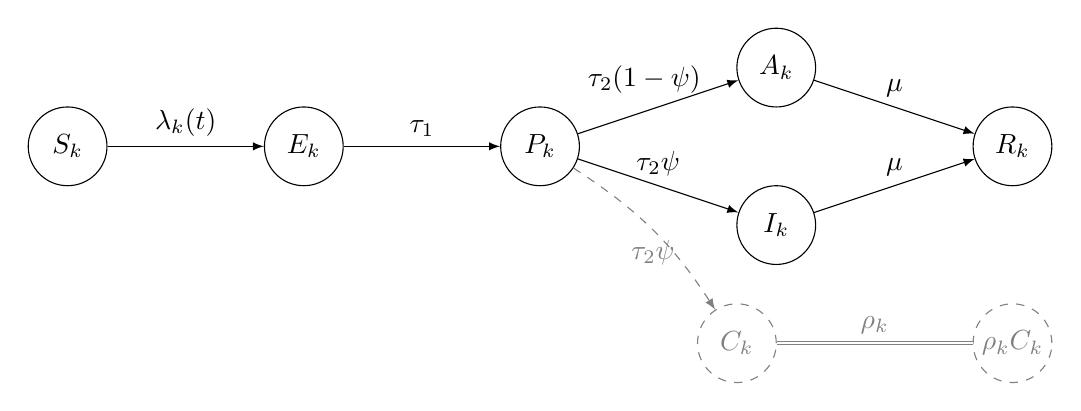
\begin{tikzpicture}
				% cascade of care
				\node[circle, draw, inner sep=0pt, minimum size=1cm] (S) at (0,0) {$S_k$};
				\node[circle, draw, inner sep=0pt, minimum size=1cm] (E) at (3,0) {$E_k$};
				\node[circle, draw, inner sep=0pt, minimum size=1cm] (P) at (6,0) {$P_k$};
				\node[circle, draw, inner sep=0pt, minimum size=1cm,gray,dashed] (C) at (8.5,-2.5) {$C_k$};
				\node[circle, draw, inner sep=0pt, minimum size=1cm,gray,dashed] (rho_C) at (12,-2.5) {$\rho_k C_k$};
				\node[circle, draw, inner sep=0pt, minimum size=1cm,fill=white] (I) at (9,-1) {$I_k$};
				\node[circle, draw, inner sep=0pt, minimum size=1cm] (A) at (9,1) {$A_k$};
				\node[circle, draw, inner sep=0pt, minimum size=1cm] (R) at (12,0) {$R_k$};
				
				\draw[->,>=latex] (S) edge node[above] { $\lambda_k(t)$} (E);
				\draw[->,>=latex] (E) edge node[above] { $\tau_1$ } (P);
				\draw[->,>=latex] (P) edge node[yshift=10,xshift=-5] { $\tau_2(1-\psi)$ } (A);
				\draw[->,>=latex] (P) edge node[above] { $\tau_2\psi$ } (I);
				\draw[->,>=latex,gray,dashed] (P) edge[bend left=12] node[below] { $\tau_2\psi$ } (C);
				\draw[->,>=latex] (A) edge node[above] { $\mu$ } (R);
				\draw[->,>=latex] (I) edge node[above] { $\mu$ } (R);
				\draw[double,gray] (C) -- node[above] { $\rho_k$ }  (rho_C);
			\end{tikzpicture}
		}
	\end{figure}
	\begin{itemize}	
	\item[-] dummy compartment $C_k(t)$ records the cumulative incidence of symptomatic infections for each age group $k$
	$$
		\frac{dC_k}{dt} = \tau_2 \psi P_k
		$$
\end{itemize}
\end{itemize}
	
	
}


\frame{
	\frametitle{Model development}

\begin{itemize}
	\item new symptomatic infections by day of symptom onset by age:
	$$
		\Delta C_{k,t} =  C_k(t) - C_k(t-1) 
	$$
	\item \alert{new reported infections} per day of symptom onset, introducing the age-specific \alert{ascertainment proportion $\rho_k$}:
	$$
		A_t = \sum_k^9 \rho_k \Delta C_{k,t}^{I}
		\label{eq:g}
	$$
	\item the \alert{age distribution} of all reported cases up to $t_{\text{max}}$ :
	$$
		B_k =  \frac{\rho_k C^I_k(t_{\text{max}})}{\sum_k^9 \rho_k C^I_k(t_{\text{max}})}
	$$

\end{itemize}
}
\frame{
	\frametitle{Model development}

\begin{itemize}

	\item $A_t$ can be mapped to \alert{reported incidence data $\mathds{A}$} using a negative binomial likelihood:
	$$
	\Pr(\theta| \mathds{A}) =  \prod_{t=t_1}^{t_{\text{max}}} \text{Neg-Bin}(\mathds{A}_t| A_t,\phi_1)	
	$$
	
	\item $B_k$ can be mapped to the \alert{age distribution of reported cases $\mathds{B}$} using a multinomial likelihood:
	$$
		\Pr(\theta| \mathds{B}) = \text{Multinomial}(\mathds{B}_1,\ldots,\mathds{B}_9|B_1,\ldots,B_9)
	$$
\end{itemize}
}



\frame{
	\frametitle{Model development}
	Model fit to deaths:
	\begin{itemize}
		\item mortality is considered outside of the system of ODEs, using an age-specific \alert{mortality parameter $\varepsilon_k$} (probability of death given \textit{symptomatic} infection)
		\item we account for the delay with a discretized log-normal distribution of time from symptom onset to death $\mathds{I}$ of length 60 
	\begin{figure}
		\centering
		\includegraphics[width=.6\linewidth]{example_hauser/distribution_onset_to_death.pdf}
	\end{figure}

\end{itemize}
}
	
	
\frame{
	\frametitle{Model development}
	\begin{itemize}
		\item deaths in age group $k$ at time $t$ ($1\leq t \leq t_{\text{max}}+60$) among people infected up to $t_{\text{max}}$:
		$$
			M_{k,t}= \varepsilon_k\sum_d^{60}  \Delta C_{k,t-d} \mathds{I}_d 
			\label{eq:h}
		$$
		\item deaths summed over age groups, assuming that all deaths are reported:
		$$
			M_{t}= \sum_k^9 M_{k,t}
		$$
			\item the \alert{age distribution of all deaths} occurring up to $t_{\text{max}}$:
		$$
		D_k = \frac{\sum_{t=1}^{t_{\text{max}}} M_{k,t}}{ \sum_{t=1}^{t_{\text{max}}} M_{t}}
		$$
	\end{itemize}
}


\frame{
	\frametitle{Model development}
	\begin{itemize}
	\item $M_t$ can be mapped to \alert{daily death data $\mathds{C}$} using a negative binomial likelihood:
	$$
	\Pr(\theta| \mathds{C}) =  \prod_{t=t_1}^{t_{\text{max}}} \text{Neg-Bin}(\mathds{C}_t|M_t,\phi_2)
	$$
	
	\item $D_k$ can be mapped to the \alert{age distribution of deaths $\mathds{D}$} using a multinomial likelihood:
	$$
		\Pr(\theta| \mathds{D}) = \text{Multinomial}(\mathds{D}_1,\ldots,\mathds{D}_9|D_1,\ldots,D_9)
	$$
	\end{itemize}
	\bigskip
	This leads to the following joint likelihood:
	$$
	\Pr(\theta | \mathds{A},\mathds{B},\mathds{C},\mathds{D}) = \Pr(\theta| \mathds{A}) \cdot \Pr(\theta| \mathds{B}) \cdot \Pr(\theta| \mathds{C}) \cdot \Pr(\theta| \mathds{D})
	$$
	
	with  $\theta=\{\beta, \eta, \xi, \nu, \psi, \pi, \rho_k, \varepsilon_k, \phi_1, \phi_2 \}$.
}



\frame{
	\frametitle{Model development}
	Last bits:
	\begin{itemize}
		\item there is an \alert{identifiability issue with $\rho$}
		\item[$\rightarrow$] fix $\rho_9$ (for 80+) to 100\%, assuming that all symptomatic infections among very high risk persons will be reported
		\bigskip
		\item some \alert{remaining unknowns} (data correction in China, role of children, lower $\rho_9$...)
		\item[$\rightarrow$] sensitivity analyses
	\end{itemize}
}


\frame{
	\frametitle{Inference}
	You know the drill:
	\begin{itemize}
		\item set priors
		\item prior predictive check
		\item sampling (on high performance computing cluster $\sim$ 2h)
		\item basic diagnostic tests
		\item examine trace plots and chains
		\item posterior predictive check
	\end{itemize}
}


\frame{
	\frametitle{Results in Hubei}
	Posterior predictive check (Hubei):
		\begin{figure}
		\centering
		\includegraphics[width=1\linewidth]{example_hauser/supp_fit_16B.pdf}
	\end{figure}
	
}


\frame{
	\frametitle{Results in Hubei}
	Ascertainment (posteriors of $\rho_k$):
	\begin{figure}
		\centering
		\includegraphics[width=.7\linewidth]{example_hauser/ascertainment.png}
	\end{figure}
	
}

\frame{
	\frametitle{Results in Hubei}
	Mortality among symptomatics or sCFR (posteriors of $\varepsilon_k$):
	\begin{figure}
		\centering
		\includegraphics[width=.7\linewidth]{example_hauser/scfr.png}
	\end{figure}
	
}

\frame{
	\frametitle{Results in Hubei}
	Effect on the assumption on $\rho_9$ on IFR estimate:
	\begin{figure}
		\centering
		\includegraphics[width=.7\linewidth]{example_hauser/rho9.png}
	\end{figure}
	
}

\frame{
	\frametitle{Results in all regions}
	Posterior predictive check (Spain):
	\begin{figure}
		\centering
		\includegraphics[width=1.01\linewidth]{example_hauser/supp_fit_spain.pdf}
	\end{figure}
	
}

\frame{
	\frametitle{Results in all regions}
	\alert{IFR estimates} (compared to CFR and sCFR)
	\begin{figure}
		\centering
		\includegraphics[width=.7\linewidth]{example_hauser/ifr_all.png}
	\end{figure}
	
}
\frame{
	\frametitle{Results in all regions}
	\alert{IFR estimates} by age
	\begin{figure}
		\centering
		\includegraphics[width=.7\linewidth]{example_hauser/ifr_age_all.png}
	\end{figure}
	
}
\frame{
	\frametitle{Conclusions}
	\begin{figure}
		\centering
		\includegraphics[width=\linewidth]{example_hauser/table_res.png}
	\end{figure}
	\begin{itemize}
		\item IFR estimates adjusted for under-ascertainment and right-censoring are \alert{more similar across countries} than CFR
		\item still some degree of \alert{heterogeneity}
		\item clear \alert{increase of mortality with age}
	\end{itemize}
}
\frame{
	\frametitle{Conclusions}
	General comments:
	\begin{itemize}
		\item knowing the \alert{data-generating mechanisms} to avoid misinterpretation
		\item this knowledge can be used to build a model to adjust for known biases
		\item estimates of IFR obtained \alert{early in the epidemic}, mostly confirmed in later seroprevalence studies
	\end{itemize}
}


\frame{
	\frametitle{Acknowledgements \& ressources}
	\begin{itemize}
		\item Stan forums \\ \url{https://discourse.mc-stan.org/}
		\item Michael Betancourt, \textit{Introduction to Stan} \\ \url{https://betanalpha.github.io/assets/case_studies/stan_intro.html}
		\item Andrew Gelman et al., \textit{Bayesian workflow} \\ \url{https://arxiv.org/abs/2011.01808}
		\item Chi Feng, \textit{MCMC interactive gallery} \\ \url{https://chi-feng.github.io/mcmc-demo/app.html}
		\item Daniel Lee, \textit{ODEs in Stan} \\ \url{https://youtu.be/hJ34_xJhYeY}
%		\item Richard McElreath, \textit{Statistical rethinking} \url{https://youtu.be/4WVelCswXo4}
	
	\end{itemize}
}


\end{document}
